\documentclass[../main.tex]{subfiles}

\begin{document}
\subsection{The reactive manifesto}
As mentioned in the introduction each today's systems have to handle big loads of data, coming from thousands of concurrent users, which are demanding low latency responses by terms of milliseconds and robust systems with a 100\% of up time.

The reactive manifesto \autocite{2014TheManifesto} calls Reactive Systems the ones able to cope with this expectances and gives this description: "Reactive Systems are more flexible, loosely-coupled and scalable. This makes them easier to develop and amenable to change. They are significantly more tolerant of failure and when failure does occur they meet it with elegance rather than disaster. Reactive Systems are highly responsive, giving users effective interactive feedback."

%% Consider talking about https://www.lightbend.com/blog/why-do-we-need-a-reactive-manifesto

At the same time it describes what the traits of reactive systems are. This traits can be categorised hierarchically by the end goal they serve. Being responsiveness the trait which directly provides value to systems and the other three characteristics that reactive systems need to meet in order to be responsive. This relationship can be visualised in the Figure \ref{fig:reactive}.

\begin{figure}[ht]
    \centering
        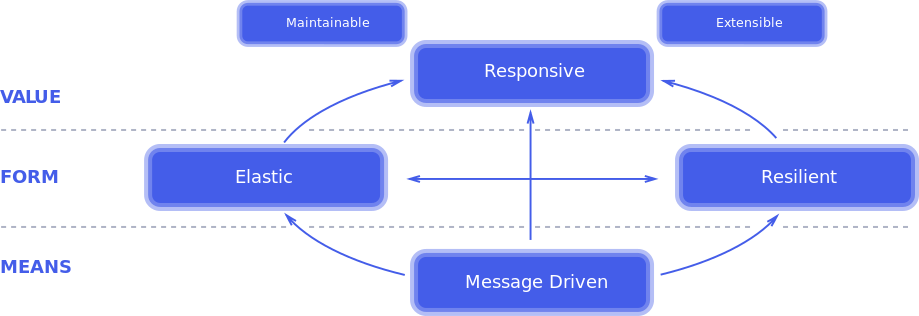
\includegraphics[width=1\textwidth]{images/reactive-traits.png}
    \caption{A hierarchical view at the reactive principles.}
    \label{fig:reactive}
\end{figure}

\subsection{The reactive principles}
\subsubsection{Responsive}
Responsiveness is the cornerstone of the reactive systems. Systems which are responsive are more comfortable to use for users as they respond faster and adapt quicker to their needs.

Google found out in 2007 that additional 0.5 seconds of load time of a search could lead to a loss of interest of on the search of a 20\%. %% https://www.youtube.com/watch?v=BQwAKsFmK_8

More recently in an study developed by Akamai Technologies in 2017 other insights about consequences of pages responsiveness, being some of the most interesting.

\begin{itemize}
    \item A 100-millisecond delay in website load time can hurt conversion rates by 7 percent 

    \item A two-second delay in web page load time increase bounce rates by 103 percent

    \item 53 percent of mobile site visitors will leave a page that takes longer than three seconds to load
    
    \item Bounce rates were highest for mobile phone shoppers, while tablet shoppers had the lowest bounce rate
\end{itemize}

\end{document}